\section{Worked Gaussian and infinite-horizon analyses}\label{sec:example}

Table~\ref{tab:params} specifies parameters for the canonical Gaussian learning environment, matching the first and second prior moments of the baseline political primitives[cite: 1]. Because Gaussian updating eliminates interval-endpoint kinks, the transitional mandate schedule is globally smooth on $(S_-,S_+)$ while preserving exact closed-form expressions under fixed electoral odds and smooth quadrature under belief-responsive voting.

\begin{table}[htbp]\centering\small
\caption{Parameter values for the Gaussian worked analysis}\label{tab:params}
\begin{tabular}{@{}p{.27\linewidth}p{.66\linewidth}@{}}
\toprule
Object & Specification\\ \midrule
Persistent returns & $\alpha\sim\mathcal N(0,\,v_\alpha)$ with $v_\alpha=.01$ ($\sigma_\alpha=.10$); $\beta\sim\mathcal N(.50,\,v_\beta)$ with $v_\beta=.25$ ($\sigma_\beta=.50$), independent.\\
State and monitoring & $\omega_t=\pm 1$ with equal probabilities ($\sigma_\omega^2=1$). Within-term report reveals $\omega_t$ with probability $S_t$ and gives $m_t=0$ otherwise. Outcome error $\varepsilon_t\sim\mathcal N(0,\,\sigma_\varepsilon^2)$ with $\sigma_\varepsilon=.25$.\\
Party preferences & $(d_L,\gamma_L^P)=(-.5,-2)$ and $(d_R,\gamma_R^P)=(1.5,2)$, so $\Dd=2$ and $\Gamma_L=\Gamma_R=2$.\\
Campaign menus & $w_L=-\ell$ and $w_R=r$, with $\ell,r\in[0,1]$ ($\bar\ell=\bar r=1$) in two-election comparisons and $\ell,r\in\{0,1\}$ in infinite-horizon comparisons.\\
Voters and valence & Equal cohort weights ($\nu=.5$). Swing voter type $(d_v,\gamma_v)=(.505,1)$. Valence takes $-100,0,100$ (or partisan-loyalist equivalents in term $2$) with probabilities $.45,.10,.45$.\\
Civic enforcement & Long-lived blocs of types $(-.5,0)$ and $(1.5,0)$; endorsement cost $c=.5$; quorums of $1$ and $2$ equally likely ($q=1/2$).\\
Discounting and costs & $\delta=.25$. Transitional game uses $k=2.40$, current $S\in[0,1]$, and consolidated term-$2$ monitoring $S_2=.05$.\\
\bottomrule
\end{tabular}
\end{table}

\subsection{Single-election benchmarks and four-regime voter realignment}

Consider first the cross-pressured voter $(d_v,\gamma_v)=(.45,1)$ at the prior $(a,b)=(0,1/2)$[cite: 1]. Under full mandates $(\ell,r)=(1,1)$, this voter prefers Left's ordinary baseline by $\Delta_v^z=-.20$ in squared-loss units while sharing Right's responsiveness slope, yielding $\Delta_v(1,1;S)=-.20+S$ and ex ante realignment at $S=.20$[cite: 1].

Allowing this cross-pressured voter $(.45,1)$ to cast the neutral ballot in the single-election campaign game (with $k=2.15$ so transfer thresholds lie inside $(0,1)$) illustrates Proposition~\ref{prop:realign} in closed form. Right uniquely offers $r^*=1$ for every $S>0$, while Left faces the incumbent-appeasement bound $\ell_{\mathrm{tr}}(S)=\sqrt{1+1.20/S}-2$ and the voter-retention bound $\ell_{\mathrm{vo}}(S)=\sqrt{.80/S}-1$:
\[
 \ell^*(S)=
 \begin{cases}
 1, & 0<S\le .15 \quad (p^*=.55,\ \text{concede}),\\
 \sqrt{1+1.20/S}-2, & .15<S\le .40 \quad (p^*=.55,\ \text{concede}),\\
 \sqrt{.80/S}-1, & .40<S\le .80 \quad (p^*=.55,\ \text{refuse}),\\
 1, & .80<S\le 1 \quad (p^*=.45,\ \text{refuse}).
 \end{cases}
\]
Across $(.15,.40]$, Left moderates steeply to buy peaceful turnover even though its electoral odds are safe at $.55$. Once $S$ crosses $.40$, compliance breaks down and $\ell^*(S)$ jumps upward from $0$ to $\sqrt{2}-1\simeq .414$ to retain the swing voter under refusal; once $S$ crosses $.80$, the swing voter realigns to $R$ and $\ell^*(S)$ jumps a second time to $1$.

Returning to Table~\ref{tab:params} with $(d_v,\gamma_v)=(.505,1)$ and $k=2.40$, Left's certificate probability is fixed at $p=.45$ and $T_{R,1}(\ell,r;S)=-.40+(S/8)(4r-r^2+4\ell+\ell^2)$[cite: 1].

\begin{result}[Single-election accommodation]\label{cor:onet}
With one election and $S>0$ under Table~\ref{tab:params}, the unique campaign equilibrium has $r^*=1$, $\ell_1^*(S)=1$ for $0<S\le .40$, and $\ell_1^*(S)=\sqrt{1+3.2/S}-2$ for $.40<S\le 1$, with concession throughout $[0,1]$. If mandate restrictions are removed ($w_L,w_R\in\mathbb R$, Proposition~\ref{prop:unconstrained}), Left crosses zero at $S_0=.80$, adopts a pro-incumbent crisis slope $w_L^*(S)=2-\sqrt{.80/S}>0$ on $(.80,4.3166]$, and endogenously abandons capitulation above $S^{**}\simeq 4.3166$ whenever $\sigma_\omega^2>S^{**}$.
\end{result}

\subsection{Transitional elections under smooth Gaussian learning}

Now add the consolidated second election ($S_2=.05$) under Table~\ref{tab:params}. Here $c_0=v_\alpha+\sigma_\omega^2 v_\beta=.26$, $Q_2=v_\alpha^2+S_2\sigma_\omega^2 v_\beta^2=.003225$, and $\psi(x)=x^2/(.26x^2+.0625)$. Compare the single-term game against three dynamic benchmarks at a flat opposition mandate $(\ell,r)=(0,1)$:
\begin{align}
 T_{R,1}(0,1;S) &= -.40+.375S,\nonumber\\
 T_{R,2}^{\mathrm{nl}}(0,1;S) &= -.1678125+.375S,\nonumber\\
 T_{R,2}^{f}(0,1;S) &= -.161735+.374822S,\nonumber\\
 T_{R,2}^{o}(0,1;S) &= -.154989+.374822S.
 \label{eq:flatcompare}
\end{align}
Applying the three-way decomposition \eqref{eq:threedecomp} at $S=0$ separates the $+.245011$ dynamic shift between $T_{R,1}$ and $T_{R,2}^o$ into exact substantive channels:
\begin{enumerate}
\item \emph{Horizon (regime-persistence) effect:} $q\delta G_2^{\mathrm{nl}}(.55)=.125(1.8575)=+.2321875$, lowering the upper transfer cutoff from above $1$ in the one-election game to $\overline S^{\mathrm{nl}}=.447500$ without any learning.
\item \emph{Policy-adaptation learning effect:} $+.0060775$ (at $S=0$), reflecting the net informational value of trials at fixed term-$2$ election odds $\pi_2=.55$ (where $\kappa_R(.55)=-.60<0$), lowering the upper cutoff to $S_+^f\simeq .431498$.
\item \emph{Electoral-realignment learning effect:} $+.0067457$, reflecting the risk that Left's trial produces a negative posterior intercept realization $a'(Z)<0$ that swings the term-$2$ neutral voter to Left, lowering Right's expected lawful return probability from $.550000$ to $.535858$ and pulling the upper cutoff down further to $S_+^o\simeq .413501$.
\end{enumerate}
Consequently, holding the two-election horizon and all institutional parameters fixed, **pure Bayesian learning flips peaceful turnover into refusal and platform polarization across the entire interval $S\in(.413501,.447500]$.**

\begin{result}[Smooth Gaussian mandates and breakdown]\label{prop:two}
In the two-election Gaussian game of Table~\ref{tab:params} under ordinary belief-responsive voting ($o$), let $\underline S\simeq .155045$ and $\overline S\simeq .413501$. For every $S>0$, the unique transitional campaign has $r^*=1$ and smooth, strictly decreasing interior moderation $\ell_2^*(S)=(S_o^\dagger)^{-1}(S)$ on $(\underline S,\overline S]$, with $\ell_2^*(S)=1$ on $(0,\underline S]\cup(\overline S,1]$. Incumbent $R$ concedes on $[0,\overline S]$ and refuses defeat on $(\overline S,1]$, where Left's installation probability drops from $.45$ to $.225$.
\end{result}

\begin{figure}[htbp]\centering
\IfFileExists{mandates_and_transfer.pdf}{%
  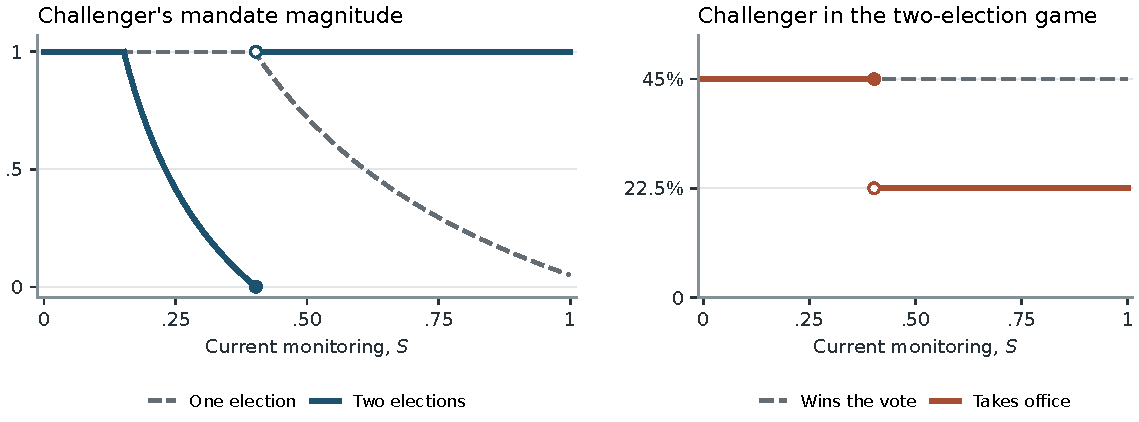
\includegraphics[width=.98\linewidth]{mandates_and_transfer.pdf}%
}{%
  \begin{tikzpicture}[scale=0.94]
    \begin{scope}
      \draw[->, thick] (0,0) -- (5.3,0) node[right,font=\scriptsize] {$S$};
      \draw[->, thick] (0,0) -- (0,3.35) node[above,font=\scriptsize] {Left responsiveness $\ell^*(S)$};
      \draw[dashed, inkblue!65, thick] (0,3) -- (2.0,3);
      \draw[dashed, inkblue!65, thick, domain=0.40:1.0, samples=50]
        plot ({5*\x}, {3*(sqrt(1+3.2/\x)-2)});
      \draw[thick, inkblue] (0,3) -- (0.775,3);
      \draw[thick, inkblue, domain=0.155045:0.413501, samples=50]
        plot ({5*\x}, {3*(sqrt(1+1.2406/\x)-2)*0.992});
      \draw[thick, inkblue] (2.068,3) -- (5.0,3);
      \draw[dotted, gray] (2.068,0) -- (2.068,3);
      \fill[inkblue] (2.068,0) circle (1.9pt);
      \node[below,font=\scriptsize] at (0.78,0) {$\underline S$};
      \node[below,font=\scriptsize] at (2.07,0) {$\overline S$};
      \node[below,font=\scriptsize] at (5.0,0) {$1$};
      \node[left,font=\scriptsize] at (0,3) {$1$};
      \node[font=\scriptsize, inkblue!75] at (3.7,0.65) {1 election};
      \node[font=\scriptsize, inkblue] at (3.6,2.68) {2 elections (Gaussian)};
    \end{scope}
    \begin{scope}[xshift=6.8cm]
      \draw[->, thick] (0,0) -- (5.3,0) node[right,font=\scriptsize] {$S$};
      \draw[->, thick] (0,0) -- (0,3.35) node[above,font=\scriptsize] {Prob. of taking office};
      \draw[dashed, gray, thick] (0,2.45) -- (5.0,2.45) node[right,font=\scriptsize] {$.45$ (certified)};
      \draw[thick, inkblue] (0,2.45) -- (2.068,2.45);
      \draw[thick, inkblue] (2.068,1.225) -- (5.0,1.225) node[right,font=\scriptsize] {$.225$ (installed)};
      \fill[inkblue] (2.068,2.45) circle (1.9pt);
      \node[below,font=\scriptsize] at (2.07,0) {$\overline S$};
      \node[below,font=\scriptsize] at (5.0,0) {$1$};
    \end{scope}
  \end{tikzpicture}%
}
\caption{Equilibrium opposition mandates (left) and probability of taking office (right) across monitoring precision $S$ under Gaussian learning. Filled dots indicate equilibrium behavior at $S=\overline S\simeq .4135$.}\label{fig:mandates}
\end{figure}

\subsection{Isolating ex post electoral realignment}

Comparing ordinary term-$2$ voting ($o$) directly against the fixed-neutral counterfactual ($f$, Corollary~\ref{cor:family}) isolates how ex post voter realignment alters today's transfer decision.

\begin{result}[Electoral use of a Gaussian trial]\label{cor:feedback}
At $S=.42$ and $k=2.40$ in Table~\ref{tab:params}, ordinary belief-responsive term-$2$ voting induces $(\ell^*,r^*)=(1,1)$ today and Right refuses defeat ($T_{R,2}^o(0,1)=+.002436>0$). Under the fixed-neutral counterfactual ($\pi_2=.55$ fixed), Right chooses $r^*=1$, Left moderates to $\ell^*\simeq .020419$, and Right concedes ($T_{R,2}^f(0,1)=-.004310<0$).
\end{result}

\subsection{Repeated elections under Gaussian Kalman filtering}

Now consider the infinite-horizon game with binary mandates $\ell,r\in\{0,1\}$ and permanent monitoring $S\in\{.05,.14\}$ at $k=2.55$. First, Proposition~\ref{prop:infinite} constrains equilibrium behavior analytically before any numerical computation: at the prior ($\sigma_\alpha=.10,\sigma_\beta=.50$), the discounted parameter-uncertainty slack $\delta\mathcal U_I(h_0)/(1-\delta)$ is only $.030$ at $S=.05$ and $.060$ at $S=.14$, and vanishes altogether ($\mathcal U_I(h)\to 0$) as Kalman filtering resolves $(\alpha,\beta)$. Consequently, Proposition~\ref{prop:infinite} alone (with $\underline\pi_J=.45$) certifies refusal in \emph{every} stationary MPE at high-slope, positive-intercept posteriors such as $(a,b)\to(+.02,1)$ ($T_I\ge +.01694$ at $S=.05$ and $+.39719$ at $S=.14$).

Solving the stationary MPE correspondence via backward precision induction on a Gauss-Hermite Kalman posterior grid (Appendix~\ref{app:stationary}) reveals three dynamic phenomena that finite two-period games cannot capture together[cite: 1]:

\begin{result}[Learning reversals, reciprocal multiplicity, and takeover risk]\label{prop:stationary}
At $k=2.55$ under binary mandates:
\begin{enumerate}
\item \emph{Non-monotonic compliance reversals along a single learning path:} Starting from the prior $(a_0,b_0)=(0,.50)$ at $S=.05$, both incumbents concede defeat. If early trials reveal high crisis leverage ($b_1\approx 1.00$ with $a_1\approx 0$), policy stakes rise and both parties switch to refusal. If subsequent trials under continued democracy reveal a negative baseline return ($a_2\approx -.02,b_2\approx 1.00$), ordinary-policy moderation lowers rival distance and both parties revert to peaceful concession.
\item \emph{Reciprocal multiplicity at converged beliefs:} At converged posteriors around $(a,b)=(+.02,0)$, two stationary MPE coexist: a self-enforcing democratic equilibrium in which both parties concede because each expects its own future victories to be honored ($T_L\simeq -.0394,T_R\simeq -.1101$), and a mutual-refusal trap in which each refuses because future victories would be blocked ($T_L\simeq +.1217,T_R\simeq +.0870$).
\item \emph{Uniform increase in eventual autocratic absorption:} Raising permanent monitoring from $S=.05$ to $S=.14$ flips prior compliance from concession to refusal and raises long-run takeover risk across the entire equilibrium set (Table~\ref{tab:risk}), unlike comparative statics that require global monotonicity restrictions \citep{milgromroberts}.
\end{enumerate}
\end{result}

\begin{table}[htbp]\centering\small
\caption{Probability of eventual autocratic takeover from the prior ($k=2.55$, Kalman MPE)}\label{tab:risk}
\begin{tabular}{@{}llrr@{}}
\toprule
Permanent $S$ & Equilibrium selection at multiplicity region & Initially $L$ & Initially $R$\\ \midrule
$.05$ & Mutual concession & 23.63\% & 23.63\%\\
$.05$ & Mutual refusal    & 61.09\% & 61.09\%\\
$.14$ & Mutual concession & 58.87\% & 55.26\%\\
$.14$ & Mutual refusal    & 74.28\% & 70.43\%\\ \bottomrule
\end{tabular}
\end{table}

\section{Empirical implications and South Korean narratives}\label{sec:discussion}

Standard spatial models attribute pre-electoral moderation to competition for undecided voters. Here, identical platform restraint can instead represent a turnover tribute paid to a defeated incumbent and its supporters. Three empirical signatures distinguish this mechanism: (i) opposition restraint on crisis responsiveness ($w_L\to 0$) while preserving redistributive baselines ($d_L$) even when the opposition leads comfortably in the polls ($p$ high and flat); (ii) an abrupt upward jump back to polarized platforms precisely when compliance breaks down ($S>S_+$); and (iii) heightened refusal risk when a successor's policy trial is expected to realign future swing voters.

\paragraph{Experimental and measurement designs.}
Survey and behavioral designs can separate beliefs, responsiveness preferences, and transfer incentives directly[cite: 1]. First, eliciting outcome forecasts $Y$ at two instrument levels across calm and crisis states identifies perceived slope $b$ under \eqref{eq:dgp}, while eliciting ideal instruments at each state recovers $\gamma_i$ independently of beliefs[cite: 1]. Second, a $2\times 3\times 2$ incentivized laboratory experiment can cross (a) \emph{automatic installation} ($k=\infty$) versus \emph{costly refusal} ($k$ interior, $q=1/2$) at fixed win probability $p=.45$, (b) \emph{low, intermediate, and high forecast precision} ($S<S_-$, $S_-<S<S_+$, $S>S_+$), and (c) \emph{belief-responsive} versus \emph{fixed-certificate} second-period voting. Our theory predicts a V-shaped opposition mandate across $S$ exclusively in the costly-refusal arm, and earlier breakdown when second-period votes respond to the first-period trial.

\paragraph{Within-country evidence from South Korea.}
Comparing pivotal junctures within South Korea---holding constant a centralized presidential executive while varying crisis predictability ($S$) and civic enforcement ($q$)---illustrates all three regions of Figure~\ref{fig:phase}:

\begin{enumerate}
\item \emph{Pacted moderation to secure historic turnover ($S\in(S_-,S_+]$, December 1997):} South Korea's December 1997 presidential election coincided with an acute sovereign-liquidity crisis and IMF intervention, sending within-term policy leverage ($Sb^2$) surging just as conservative ruling elites faced the prospect of handing executive and security institutions to opposition leader Kim Dae-jung for the first time. Critically, ruling-camp splits had already given Kim a durable polling lead ($p$ high), so standard vote-seeking logic alone struggled to explain a late conservative pivot. Yet after initially floating renegotiation of the IMF package, Kim publicly pledged unconditional adherence to IMF fiscal-monetary orthodoxy and backed central-bank independence before election day---preserving his welfare-state baseline ($d_L$) while tying his crisis-intervention slope ($w_L\to 0$). Lowering delegation risk facilitated immediate post-election cooperation through a joint emergency economic committee with outgoing President Kim Young-sam, peaceful inauguration, and a consequential policy record for subsequent electorates.
\item \emph{Endogenous civic enforcement ($q$) and pre-election restraint (2024--2025):} Whereas the model's transfer node follows an electoral loss, executive self-coups during a term test the same civic-enforcement calculus ($C_i-A_i\ge c$)[cite: 1]. Following President Yoon Suk Yeol's December 2024 martial-law decree, three Gallup Korea waves tracked impeachment support: on December 10--12, 97 percent of Democratic Party identifiers and 27 percent of ruling People Power Party identifiers favored impeachment (75 percent overall); by January 7--9 and February 11--13, ruling-party support fell to 15 and 10 percent against 99 and 98 percent among opposition identifiers (64 and 57 percent overall).\footnote{Weighted percentages from Gallup Korea Daily Opinion reports \refsource{https://www.gallup.co.kr/dir/GallupKoreaDaily/GallupKoreaDailyOpinion_606(20241213).pdf}{606}, \refsource{https://www.gallup.co.kr/dir/GallupKoreaDaily/GallupKoreaDailyOpinion_608(20250110).pdf}{608}, and \refsource{https://www.gallup.co.kr/dir/GallupKoreaDaily/GallupKoreaDailyOpinion_611(20250214).pdf}{611}; see also the \refsource{https://www.loc.gov/item/global-legal-monitor/2025-05-13/south-korea-constitutional-court-upholds-presidential-impeachment/}{US Library of Congress} on the Constitutional Court ruling[cite: 1].} Initial cross-partisan defection drove $q\to 0$, blocking martial law. As attention shifted toward an impending early presidential election and the policy stakes of an opposition presidency ($A_R-C_R$), partisan enforcement polarized sharply (from a 70- to an 88-point gap)---and precisely during this window, the heavily favored opposition leadership repealed a scheduled financial-investment income tax and pledged regulatory and tax restraint ($w_L\to 0$) to reassure conservative and business constituencies ahead of the transition.
\item \emph{Polarization and autocratic closure versus mass enforcement (1971--1972 versus 1987):} Conversely, after the 1971 presidential election demonstrated surging opposition viability on a redistributive, security-reform platform ($\ell$ high, raising record risk) amid external security shocks ($S>S_+$) and high coercion capacity ($q$ high), the incumbent terminated electoral competition altogether under the 1972 Yushin constitution to pursue permanent developmental priorities ($\gamma_R^P$). By contrast, in June 1987 cross-class white-collar mobilization expanded the enforcing coalition ($q\to 0$, shifting $k/q$ into the upper region of Figure~\ref{fig:phase}), compelling ruling elites to concede competitive direct elections.\footnote{Comparative historical cases likewise require distinguishing post-defeat refusal (United States 2020; \refsource{https://www.govinfo.gov/app/details/GPO-J6-REPORT}{US House Select Committee Report}) from term-limit coups (France 1851; \refsource{https://www2.assemblee-nationale.fr/decouvrir-l-assemblee/histoire/le-suffrage-universel/la-republique-et-le-suffrage-universel/1848-la-deuxieme-republique-met-en-place-le-suffrage-universel-masculin/le-coup-d-etat-du-2-decembre-1851}{French National Assembly}) and post-appointment consolidation (Germany 1933; \refsource{https://encyclopedia.ushmm.org/content/en/timeline-event/holocaust/1933-1938/hitler-appointed-chancellor}{USHMM})[cite: 1].}
\end{enumerate}

Ultimately, peaceful democratic turnover depends on how much discretionary authority a defeated party can bear to entrust to its rival. Better economic foresight raises the stakes of delegation even under shared facts. An opposition can often buy peaceful succession by muting its future crisis response---until rising stakes render even complete restraint insufficient, causing platform moderation and democratic compliance to collapse together.

\FloatBarrier
\begin{thebibliography}{99}\small\linespread{1.0}\selectfont
\bibitem[Bueno de Mesquita and Dziuda(2023)]{partisantraps} Bueno de Mesquita, Ethan, and Wioletta Dziuda. 2023. Partisan Traps. NBER Working Paper 31827, November. \href{https://doi.org/10.3386/w31827}{DOI}.
\bibitem[Callander(2011a)]{callgood} Callander, Steven. 2011a. Searching for Good Policies. \emph{American Political Science Review} 105(4), 643--662. \href{https://doi.org/10.1017/S0003055411000426}{DOI}.
\bibitem[Callander(2011b)]{calltrial} Callander, Steven. 2011b. Searching and Learning by Trial and Error. \emph{American Economic Review} 101(6), 2277--2308. \href{https://doi.org/10.1257/aer.101.6.2277}{DOI}.
\bibitem[Fearon(2011)]{fearon} Fearon, James D. 2011. Self-Enforcing Democracy. \emph{Quarterly Journal of Economics} 126(4), 1661--1708. \href{https://doi.org/10.1093/qje/qjr038}{DOI}.
\bibitem[Graham and Svolik(2020)]{graham} Graham, Matthew H., and Milan W. Svolik. 2020. Democracy in America? Partisanship, Polarization, and the Robustness of Support for Democracy in the United States. \emph{American Political Science Review} 114(2), 392--409. \href{https://doi.org/10.1017/S0003055420000052}{DOI}.
\bibitem[Izzo et~al.(2023)Izzo, Martin, and Callander]{izzo} Izzo, Federica, Gregory J. Martin, and Steven Callander. 2023. Ideological Competition. \emph{American Journal of Political Science} 67(3), 687--700. \href{https://doi.org/10.1111/ajps.12763}{DOI}. \href{https://www.federicaizzo.com/pdf/Ideological_Competition_FINAL_Website.pdf\#page=44}{Online appendix E.1}.
\bibitem[Milgrom and Roberts(1994)]{milgromroberts} Milgrom, Paul, and John Roberts. 1994. Comparing Equilibria. \emph{American Economic Review} 84(3), 441--459. \href{https://web.stanford.edu/~milgrom/publishedarticles/Comparing\%20Equilibria.pdf}{Authors' copy}.
\bibitem[Przeworski(1991)]{przeworski} Przeworski, Adam. 1991. \emph{Democracy and the Market}. Cambridge University Press. \href{https://www.cambridge.org/core/books/abs/democracy-and-the-market/democracy/0AA4BF19C5129B8634C501C22B5FB61B}{Publisher}.
\bibitem[Rogoff(1985)]{rogoff} Rogoff, Kenneth. 1985. The Optimal Degree of Commitment to an Intermediate Monetary Target. \emph{Quarterly Journal of Economics} 100(4), 1169--1189. \href{https://doi.org/10.2307/1885679}{DOI}.
\bibitem[Svolik(2020)]{svolik2020} Svolik, Milan W. 2020. When Polarization Trumps Civic Virtue: Partisan Conflict and the Subversion of Democracy by Incumbents. \emph{Quarterly Journal of Political Science} 15(1), 3--31. \href{https://doi.org/10.1561/100.00018132}{DOI}.
\end{thebibliography}

\clearpage
\appendix
\linespread{1.045}\selectfont

\section{Policy distance and single-election proofs}\label{app:one}

\begin{proof}[Proof of Proposition~\ref{prop:fixed}]
Write $\tau_i=d_i+\gamma_i(\alpha+\beta\omega)$. Conditional on $(h,s)$, $\E[(x-\tau_i)^2\mid h,s]=(x-z_i-\rho_i m)^2+\Var(\tau_i\mid h,s)$, where the conditional variance is policy-invariant[cite: 1]. Integrating $[(z_j-z_i)+(\rho_j-\rho_i)m]^2$ over $s$ using $\E[m]=0$ and $\E[m^2]=S$ yields \eqref{eq:distance}, $\Delta_i(w_L,w_R;S)$, and \eqref{eq:termgain}[cite: 1]. Differentiating \eqref{eq:termgain} in $S$ gives $qb^2[(w_J-\gamma_I^P)^2-(w_I-\gamma_I^P)^2]$.
\end{proof}

Omitting the policy-invariant baseline $2d_i\gamma_i(\alpha+\beta\omega)+\gamma_i^2(\alpha+\beta\omega)^2$ from squared loss---whose expected discounted sum from a common prior $h$ is independent of policy and regime by iterated expectations under finite fourth moments---gives the normalized flow for rule $\bar x=d_j+wa$[cite: 1]:
\begin{equation}
 f_i(j,w,h,S)=-(\bar x-d_i)^2+2\gamma_i\bar x a
                    +S b^2(2\gamma_i w-w^2).
 \label{eq:flow}
\end{equation}

\begin{proof}[Proof of Proposition~\ref{prop:onegen}]
Subtracting $R$'s loss under $r$ from its loss under $-\ell$ gives \eqref{eq:g-symbolic}[cite: 1]. For $v>0$, $R$'s own-victory payoff strictly increases in $r$, its concession payoff is independent of $r$, and its refusal payoff is nondecreasing in $r$; since $1-p>0$, $r^*=\bar r$ is strictly dominant[cite: 1]. Against $\bar r$, $\partial_\ell g_R(\ell,\bar r;S)=2\Dd\,a+2v(\Gamma_R+\ell)>0$, left's payoff strictly increases in $\ell$ within each compliance branch, and \eqref{eq:leftone} ranks $\ell=0$ with concession strictly above $\ell=\bar\ell$ with refusal, uniquely selecting $\ell^*(S)$[cite: 1].
\end{proof}

\begin{proof}[Proof of Proposition~\ref{prop:realign}]
At $a=0$, $\Delta_v^O=(1-q\mathbf 1_{\{T_{R,1}>0\}})\Delta_v(\ell,r;S)$ with $1-q>0$ and $\Delta_v(\ell,r;S)=\Delta_v^z+Sb^2[(\gamma_v+\ell)^2-(\gamma_v-r)^2]$. Since $0<\bar r\le\gamma_v$, increasing $r$ on $[0,\bar r]$ strictly increases $\Delta_v$ (weakly lowering $p(\ell,r;S)$), strictly raises $f_R(R,r)$, and weakly raises $\max\{0,T_{R,1}\}$. Because winning the count strictly dominates losing it for $R$ ($f_R(R,r)>f_R(L,-\ell)$ and $(1-q)[f_R(R,r)-f_R(L,-\ell)]+k>0$), $r^*=\bar r$ is strictly dominant for $S>0$.

Against $\bar r$, $\ell_{\mathrm{tr}}(S)<\ell_{\mathrm{vo}}(S)$ implies that every conceded offer ($\ell\le\ell_{\mathrm{tr}}$) retains the swing voter ($p=p_-+p_0$). Within each regime---conceded with $p_-+p_0$, refused with $p_-+p_0$, and refused with $p_-$---$L$'s payoff strictly increases in $\ell$, leaving $\min\{\bar\ell,\ell_{\mathrm{tr}}(S)\}$, $\min\{\bar\ell,\ell_{\mathrm{vo}}(S)\}$, and $\bar\ell$ as the sole candidates. Condition~\eqref{eq:leftone} selects $\min\{\bar\ell,\ell_{\mathrm{tr}}(S)\}$ on $(0,S_+^{\mathrm{tr}}]$; on $(S_+^{\mathrm{tr}},S_+^{\mathrm{vo}}]$, concession is unattainable and \eqref{eq:voterretain} selects $\min\{\bar\ell,\ell_{\mathrm{vo}}(S)\}$; above $S_+^{\mathrm{vo}}$, $\Delta_v(\ell,\bar r;S)>0$ for all $\ell\ge 0$, selecting $\bar\ell$. In Section~\ref{sec:example}'s illustration ($(.45,1)$, $k=2.15$), \eqref{eq:voterretain}'s net margin equals $29/200-9S/20+33\sqrt{5S}/200\ge .115>0$ on $[.40,.80]$.
\end{proof}

\begin{proof}[Proof of Proposition~\ref{prop:unconstrained}]
At $a=0,S>0$, $w_R=\Gamma_R$ uniquely minimizes $Sb^2(w_R-\Gamma_R)^2$ on victory and under successful refusal without affecting concession, so $w_R^*=\Gamma_R$. Against $\Gamma_R$, $T_{R,1}(w_L,\Gamma_R;S)\le 0\iff |\Gamma_R-w_L|\le K/(|b|\sqrt{S})$. Left's best conceded weight is $-\Gamma_L$ for $S\le S_-$ and $w_L^{\mathrm{tr}}(S)=\Gamma_R-K/(|b|\sqrt{S})$ for $S>S_-$ (crossing $0$ at $S_0$), while its best refused weight is $-\Gamma_L$. Writing $x=|b|\sqrt{S}G>K$ for $S>S_-$, Left's loss conditional on winning the count is $(x-K)^2$ under $w_L^{\mathrm{tr}}(S)$ versus $q(\Dd^2+x^2)$ under $-\Gamma_L$. Their difference $(1-q)x^2-2Kx+K^2-q\Dd^2$ is strictly convex, equals $-k<0$ at $x=K$, and crosses zero uniquely at $x^{**}=[K+\sqrt{q(K^2+(1-q)\Dd^2)}]/(1-q)>K$, yielding $S^{**}$. Under partial commitment \eqref{eq:partial}, minimizing $\E[(x-d_j-\gamma_j^P b m)^2\mid s]+\chi(x-d_j-w_j b m)^2$ gives $\tilde w_j(w_j)$.
\end{proof}

\section{Transitional elections and Gaussian learning proofs}\label{app:gaussian}

\begin{proof}[Proof of Proposition~\ref{prop:main}]
Linearity of expectation over the binary news draw $R^2=S/\sigma_\omega^2$ yields affine branch payoffs $W_i,A_i,C_i$ and \eqref{eq:twodecomposition}[cite: 1]. For $R^2>0$, $W_R$ strictly increases and $A_R$ is nondecreasing in $r$, making $r^*=\bar r$ strictly dominant (including against mixed offers)[cite: 1]. Against $\bar r$, Left's conditional payoffs under concession and refusal strictly increase in $\ell$ for $R^2>0$, while \eqref{eq:accommodate} makes the affine difference between $\ell=0$ (conceded) and $\bar\ell$ (refused) strictly positive across $[0,1]$[cite: 1]. By Condition~3, $D_0(\ell)\le D_0(\bar\ell)<k/q<D_1(0)\le D_1(\ell)$, so $(1-R^2)D_0(\ell)+R^2 D_1(\ell)=k/q$ defines the unique continuous, strictly decreasing schedule \eqref{eq:generalcut} and equilibrium \eqref{eq:genstar}[cite: 1].
\end{proof}

\begin{proof}[Proof of Corollary~\ref{cor:family}]
Given $(x_1,\omega_1)$ with $\omega_1^2=\sigma_\omega^2$, $Y_1-x_1(a+b\omega_1)=x_1(\alpha-a)+x_1\omega_1(\beta-b)+\varepsilon_1$ is normal with mean zero, variance $c_0 x_1^2+\sigma_\varepsilon^2$, and covariances $x_1 v_\alpha$ with $\alpha$ and $x_1\omega_1 v_\beta$ with $\beta$, establishing \eqref{eq:psi}. Thus $\E[a'\mid x_1,\omega_1]=a$ and $\E[a'^2+S_2 b'^2\mid x_1,\omega_1]=v_2(h)+Q_2\psi(x_1)$. Evaluating \eqref{eq:flow} in term $2$ at $(\bar\ell,\bar r)$ gives
\begin{align*}
 V_R^\A(R,h') &= \Gamma_R^2 v_2(h')+2\Gamma_R d_R a',\\
 V_R^\D(L,h') &= -(1-\pi_2)\Dd^2+a'\big[2\Gamma_R(\pi_2 d_R+(1-\pi_2)d_L)+2(1-\pi_2)\Dd\bar\ell\big]+\kappa_R(\pi_2)v_2(h'),\\
 V_L^\D(L,h') &= -\pi_2\Dd^2-a'\big[2\Gamma_L(\pi_2 d_R+(1-\pi_2)d_L)+2\pi_2\Dd\bar r\big]+\kappa_L(\pi_2)v_2(h').
\end{align*}
Taking expectations over $Z\sim\mathcal N(0,1)$ cancels all linear-$a'$ differences from $K_j^e V-V(h)$ and simplifies $V_R^\A(R,h)-V_R^\D(L,h)=G_2^{\mathrm{nl}}(\pi_2)$, yielding \eqref{eq:gaussD}. At $a=0$, $|d\Psi_j^1(w)/dw|\le |b|\sigma_\omega\bar\psi'$ and $d\Psi_j^0/dw=0$. Hence $\partial_r W_{R,1}\ge 2\sigma_\omega^2 b^2(\Gamma_R-\bar r)-\delta Q_2|\kappa_R|\sigma_\omega|b|\bar\psi'>0$, $\partial_r A_{R,1}\ge 2\sigma_\omega^2 b^2(\Gamma_R-\bar r)-\delta Q_2\Gamma_R^2\sigma_\omega|b|\bar\psi'>0$, $\partial_\ell C_{L,1}\ge 2\sigma_\omega^2 b^2(\Gamma_L-\bar\ell)-\delta Q_2|\kappa_L|\sigma_\omega|b|\bar\psi'>0$, and $D_1'(\ell)\ge 2\sigma_\omega^2 b^2(\Gamma_R+\ell)-\delta Q_2|\kappa_R|\sigma_\omega|b|\bar\psi'>0$ (matching the sufficient inequalities after dividing by $\sigma_\omega>0$ when $|b|\le 1$, or multiplying the right-hand side by $|b|/\sigma_\omega$ in general; for $a\ne 0$, adding $2a^2(\Gamma_j-\bar w_j)>\delta Q_2|\kappa_j|\,|a|\bar\psi'$ and $2\Dd\,a+2a^2\Gamma_R>\delta Q_2|\kappa_R|\,|a|\bar\psi'$ ensures strict monotonicity at $e=0$ as well). Because $\psi\in C^\infty(\mathbb R)$, $D_e\in C^\infty([0,\bar\ell])$ and implicit differentiation yields smooth $\ell^*(S)$; continuity of all strict margins in $(a,b,v_\alpha,v_\beta,\sigma_\varepsilon,d_j,\Gamma_j,k,q,\delta,S_2)$ establishes open-set persistence.
\end{proof}

\section{Infinite-horizon bound proof}\label{app:infproof}

\begin{proof}[Proof of Proposition~\ref{prop:infinite}]
In any future period $t'\ge t+1$, write $\omega_{t'}=m_{t'}+\xi_{t'}$. Conditional independence of $(\omega_{t'},s_{t'})$ from $(\alpha,\beta)$ given $\mathcal H_{t'}$ implies $\E[\xi_{t'}\mid\mathcal H_{t'},s_{t'},\alpha,\beta]=0$ and $\E[\xi_{t'}^2\mid\mathcal H_{t'}]=\sigma_\omega^2-S_{t'}$. Expanding \eqref{eq:u} at any $(\mathcal H_{t'},s_{t'})$-measurable $x_{t'}$ gives
\[
 -\E[u_I(x_{t'},\omega_{t'},\alpha,\beta)\mid\mathcal H_{t'}]
 =\Lambda_I^{j_{t'},w_{t'}}(h_{t'},S_{t'})
 +(\gamma_I^P)^2\big(\Var_{h_{t'}}(\alpha)+S_{t'}\Var_{h_{t'}}(\beta)\big)
 +(\gamma_I^P)^2\E_{h_{t'}}[\beta^2](\sigma_\omega^2-S_{t'}),
\]
where the cross term $2(\alpha-a_{t'})(\beta-b_{t'})m_{t'}$ vanishes even under correlated posteriors because $\E[m_{t'}\mid\mathcal H_{t'}]=0$ independently of $(\alpha,\beta)$. By iterated expectations ($\E[\E_{h_{t'}}[\beta^2]\mid h_t]=\E_{h_t}[\beta^2]$) and regime-independence of $\{S_{t'}\}$, the third term cancels identically between $A_I$ and $C_I$. By the law of total variance, $\E[\Var_{h_{t'}}(\theta)\mid Z_t]=\Var_{h_t}(\theta)-\Var(\E_{h_{t'}}[\theta]\mid Z_t)\le\Var_{h_t}(\theta)$ for $\theta\in\{\alpha,\beta\}$, bounding expected parameter-uncertainty loss each future period by $\mathcal U_I(h_t)$.

Under autocracy of $I$, $\Lambda_I^{I,\gamma_I^P}=0$ and attempt costs are zero, so $I$'s discounted residual continuation from $t+1$ onward lies in $[-\mathcal U_I(h_t)/(1-\delta),\,0]$. Under democracy after $I$ concedes to $J$, $J$ enters $t+1$ as incumbent and wins the $t+1$ count with probability at least $\underline\pi_J$, incurring residual loss at least $\underline\Lambda_I^J(h_t)$ while all other residual flows and attempt costs are nonpositive, bounding $I$'s democratic continuation above by $-\underline\pi_J\underline\Lambda_I^J(h_t)$. Conversely, conceding every future defeat is a feasible continuation strategy for $I$ with zero attempt costs, so Bellman optimality bounds $I$'s democratic continuation below by $-[\bar L_I(h_t)+\mathcal U_I(h_t)]/(1-\delta)$. Substituting into \eqref{eq:gain} yields \eqref{eq:infbounds}.
\end{proof}

\section{Verification of the Gaussian and Kalman worked results}\label{app:stationary}

\paragraph{Verification of Results~\ref{cor:onet}--\ref{cor:feedback}.}
Result~\ref{cor:onet} follows directly from Propositions~\ref{prop:onegen} and \ref{prop:unconstrained}: at $D=2,b=1/2,q=1/2,k=2.40$, $K=\sqrt{4.80-4}=\sqrt{.80}$ and $G=4$, giving $S_-=.80/4=.20$ under $w_j\in\mathbb R$ (or $.40$ when $\bar r=\bar\ell=1$), $S_0=.80/1=.80$, and $S^{**}=(\sqrt{.80}+\sqrt{1.40})^2/(.25\times 4)\simeq 4.3166$.

For Results~\ref{prop:two} and \ref{cor:feedback}, first verify the consolidated term-$2$ subgame at every realized posterior mean $(a',b')\in\mathbb R^2$ with $v_2=a'^2+.05b'^2>0$. For the swing voter $(.505,1)$, Right's rule $r_2=1$ yields loss $.995^2=.990025$. When $a'\ge 0$, Left's rule $l_2\in[0,1]$ yields loss $[1.005+(1+l_2)a']^2+.05b'^2(1+l_2)^2\ge 1.005^2>.995^2$, so $r_2^*=1$ guarantees $\pi_2=.55$ while uniquely maximizing $R$'s own-policy payoff, and Left uniquely plays $l_2^*=1$. When $a'<0$, $[.995+(1-r_2)|a'|]^2+.05b'^2(1-r_2)^2$ strictly decreases in $r_2$ on $[0,1]$, so $r_2^*=1$ simultaneously minimizes voter loss and maximizes $R$'s policy payoff across all $\mathbb R^2$. Against $r_2^*=1$ for $a'<0$, the swing voter's right margin is $Q_v(y)=v_2 y^2+2.01a'y+.02$ with $y=1+l_2\in[1,2]$[cite: 1]: Left plays $l_2^*=1$ whenever $Q_v(2)\le 0$ ($\pi_2=.45$) or $\min_{y\in[1,2]}Q_v(y)>0$ ($\pi_2=.55$), and otherwise compares $l_2=\min\{1,[-2.01a'+\sqrt{(2.01a')^2-.08v_2}]/(2v_2)-1\}$ ($\pi_2=.45$) against $l_2=1$ ($\pi_2=.55$).

Integrating these exact term-$2$ payoffs along \eqref{eq:psi} via 120-node Gauss-Hermite quadrature verifies Conditions~1--3 of Proposition~\ref{prop:main}:
\begin{enumerate}
\item Bloc current-term policy advantage exceeds $3.75$, while discounted term-$2$ bloc differences are bounded below $.25(4.5)<1.2$, so $C_{b_L}-A_{b_L}>2.5>.5=c$ and $C_{b_R}-A_{b_R}<-2.5$, fixing $q=1/2$. Both old and young neutral voters strictly prefer certifying $R$ across $(\ell,r)\in[0,1]^2$ (margins $\ge .02$ under concession and $\ge .01$ old / $>5.63$ young under refusal due to expected term-$2$ valence $+45$), fixing $p=.45$[cite: 1].
\item Under fixed-neutral rule $f$, Corollary~\ref{cor:family}'s slope bounds hold with wide slack ($.50>.01643$ for $R$ and $.50>.00575$ for $L$), giving $D_0^f=4.476530$, $D_1^f(0)=5.226174$, $D_1^f(1)=6.475975$, $S_-^f\simeq .161780$, and $S_+^f\simeq .431498$. Under ordinary voting $o$, $D_0^o(\ell)$ rises gently from $4.490021$ to $4.490021$ (constant at $a=0$ since $x_L(0)=-.5$), while $D_1^o(\ell)$ strictly increases from $5.239665$ at $\ell=0$ to $6.489305$ at $\ell=1$ ($\min_{\ell\in[0,1]}{D_1^o}'(\ell)>.99$), yielding $\underline S=(4.80-4.490021)/(6.489305-4.490021)\simeq .155045$ and $\overline S=(4.80-4.490021)/(5.239665-4.490021)\simeq .413501$. At $S=.42$, solving $S_f^\dagger(\ell)=.42$ gives $\ell^*\simeq .020419$.
\end{enumerate}

\paragraph{Verification of Result~\ref{prop:stationary} (Kalman MPE solver).}
Discretizing posterior means on $(a,b)\in\{-.04,-.02,0,+.02,+.04\}\times\{0,.25,.50,.75,1.00\}$ across precision stages $\tau\in\{0,1,2\}$ (with converged exact $2\times 2$ Bellman blocks $(\Id-\delta P_\tau)^{-1}u$ at $\tau=2$ and 15-node Gauss-Hermite transition kernels for $\tau<2$), bloc willingness strictly satisfies $q=1/2$ and full binary offers $(1,1)$ dominate wherever $a^2+Sb^2>0$[cite: 1]. At $\tau=2,(a,b)=(+.02,0)$, solving the two candidate compliance regimes directly yields the exact refusal gains $(T_L,T_R)=(-.039373,-.110093)$ under mutual concession and $(+.121659,+.087008)$ under mutual refusal. Propagating both equilibrium continuations backward to $\tau=0$ via $(\Id-Q)^{-1}p_A$ yields the exact absorption probabilities in Table~\ref{tab:risk} and confirms the positive-probability reversal path $(0,.50)\to(0,1.00)\to(-.02,1.00)$ at $S=.05,k=2.55$.
\end{document}